% arara: xelatex: { synctex: yes, shell: yes }
\documentclass[portuguese]{ist-thesis}

\usepackage{csquotes}
\usepackage{biblatex}
\addbibresource{main.bib}

\usepackage{lipsum}
\usepackage{booktabs}
\usepackage{tikz}
\usepackage{pgfplots}
\usetikzlibrary{positioning,arrows.meta}

\graphicspath{{graphics/}}
\pgfplotsset{table/search path = {data}}

\setcoverimage[0.6]{example-image-a}

\begin{document}

\makecover

\begin{dedication}
	I don't like sand.
\end{dedication}

\begin{acknowledgements}
	Did you ever hear the tragedy of Darth Plagueis The Wise? I thought not. It's not a story the Jedi would tell you. It's a Sith legend. Darth Plagueis was a Dark Lord of the Sith, so powerful and so wise he could use the Force to influence the midichlorians to create life... He had such a knowledge of the dark side that he could even keep the ones he cared about from dying. The dark side of the Force is a pathway to many abilities some consider to be unnatural. He became so powerful... the only thing he was afraid of was losing his power, which eventually, of course, he did. Unfortunately, he taught his apprentice everything he knew, then his apprentice killed him in his sleep. Ironic. He could save others from death, but not himself.
\end{acknowledgements}

\begin{tabstract}{Resumo, Palavras-Chave, Resumo Analítico, \textit{Abstract}}
	Resumo e palavras-chave (em português e em inglês). O resumo analítico, também designado por resumo ou abstract, descreve o objectivo, o conteúdo do trabalho e as conclusões. Deve ser escrito em português e inglês, com um máximo de 250 palavras cada e acompanhado de 4 a 6 palavras-chave.
	The abstract describes the objective, the content of the project and the conclusions. It must be written in both portuguese and english, with a maximum of 250 words, accompanied by 4 to 6 keywords.
\end{tabstract}

\tableofcontents

\listoffigures

\listoftables

\mainstart

\chapter{Introdução}

\lipsum[1]

\section{Primeira Secção}

Esta referência liga à equação \ref{eq:equation1}.

\begin{gather}\label{eq:equation1}
	\mathbb{P}\left(\frac{X_1 + \cdots + X_n}{\sqrt{n}} \leq y\right) \rightarrow \mathrm{R}(y) = \int_{-\infty}^{y} \frac{e^{-t^2/2}}{\sqrt{2\pi}}dt \qquad \mathrm{as} \quad n \rightarrow \infty
\end{gather}

\lipsum[2-3]

\begin{figure}[ht]
	\centering
	\includegraphics[width = 0.5\linewidth]{example-image}
	\caption{Imagem de exemplo.}
	\label{fig:image1}
\end{figure}

\lipsum[1]

\begin{table}[ht]
	\centering
	\begin{tabular}{c c c}\toprule
		\textbf{Expression}	& \textbf{Value of $\mathbf{x}$}	& \textbf{Value of $\mathbf{y}$}\\
		\midrule
		$y = 4x$			& $67$								& $268$							\\
		$y = x^2$			& $13$								& $169$							\\
		$y = e^x$			& $9.5$								& $33.115$						\\
		\bottomrule
	\end{tabular}
	\caption{Algumas expressões e variáveis.}
	\label{tab:tab1}
\end{table}

\lipsum[11]

\begin{figure}[ht]
	\centering
	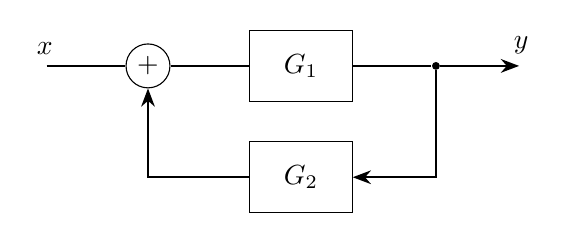
\begin{tikzpicture}
		\tikzstyle{mainblock} = [rectangle, draw, align = center, minimum height = 9mm, minimum width = 13mm];
		\tikzstyle{sum} = [circle, draw, align = center, inner sep = 2pt];
		\tikzstyle{mainpath} = [draw, thick, -{Stealth[]}];
		\node (start) at (0,0) [inner sep = 0mm, label = {90:$x$}] {};
		\node (sum1) [sum, right=of start] {$+$};
		\node (g1) [mainblock, right=of sum1] {$G_1$};
		\node (ex1) [circle, fill, inner sep = 1pt, right=of g1] {};
		\node (end) [right=of ex1, inner sep = 0mm, label = {90:$y$}] {};
		\node (g2) [mainblock, below=5mm of g1] {$G_2$};
		\path [mainpath] (start) -- (sum1) -- (g1) -- (ex1) -- (end);
		\path (ex1) -- (ex1 |- g2) [mainpath] --  (g2);
		\path (g2) -- (g2 -| sum1) [mainpath] -- (sum1);
	\end{tikzpicture}
	\caption{Exemplo de um diagrama feito em \LaTeX{}.}
	\label{fig:diag1}
\end{figure}

\lipsum[13-14]

\begin{figure}
	\centering
	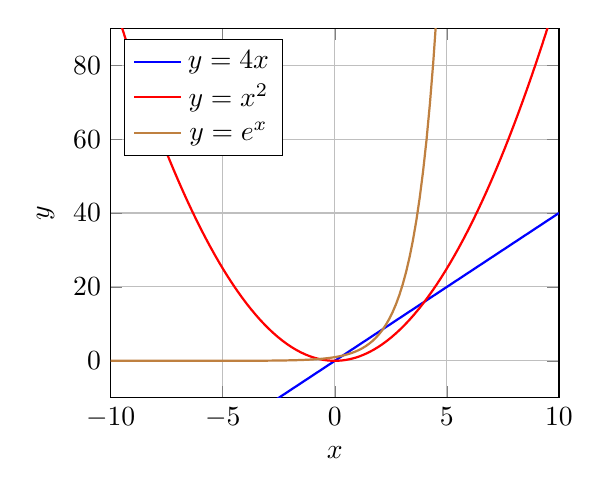
\begin{tikzpicture}
		\begin{axis}
				[width = 0.6\linewidth,
				samples = 100,
				grid = both,
				xmin = -10, xmax = 10,
				ymin = -10, ymax = 90,
				xlabel = {$x$},
				ylabel = {$y$},
				legend pos = north west,]
			\addplot [mark = none, color = blue, thick, domain = -10:10] {4*x};
			\addplot [mark = none, color = red, thick, domain = -10:10] {x^2};
			\addplot [mark = none, color = brown, thick, domain = -10:5] {e^x};
			\legend{$y = 4x$,$y = x^2$,$y = e^x$};
		\end{axis}
	\end{tikzpicture}
	\caption{Exemplo de um gráfico em \LaTeX{}.}
	\label{fig:graph1}
\end{figure}

\lipsum[15]

\begin{figure}
	\centering
	\begin{tikzpicture}
		\begin{axis}
				[width = 0.9\linewidth,
				height = 0.6\linewidth,
				xmin = 5,
				grid = both,
				xlabel = {Tempo ($x$)},
				ylabel = {Amplitude},
				legend pos = north east,]
			\addplot [red] table [col sep = comma, x index = 0, y index = 1, mark = none] {data_example.csv};
			\legend{Exemplo};
		\end{axis}
	\end{tikzpicture}
	\caption[Exemplo de um \textit{plot} de dados em \LaTeX{}.]{Exemplo de um \textit{plot} de dados em \LaTeX{}. Os dados foram obtidos de um ficheiro \texttt{.csv} auxiliar.}
	\label{fig:graph1}
\end{figure}

\lipsum

\nocite{latex-companion, fontcatalogue, latexwiki, ctan, texsx}
\printbibliography[heading = bibintoc]

\end{document}
